\section{Zielsetzung}
\label{sec:Zielsetzung}

Das Ziel dieses Versuches ist es, den Aufbau und die Funktionsweise eines
Silizium-Halbleiterdetektors aufzuzeigen und mithilfe verschiedener Messungen dessen
Eigenschaften zu untersuchen. Durch die Betrachtung der Ausleseelektronik und
der Datenverarbeitung soll zudem ein Ausblick auf größere Teilchendetektoren
gegeben werden. Schließlich wird eine $\beta^{-}$-Quelle untersucht.

\section{Theorie}
\label{sec:Theorie}
\subsection{Aufbau eines Inneren Detektors}

Die Si-Streifendetektoren sind bei großen teilchenphysikalischen Detektoren,
wie z.B. dem ATLAS-Detektor am LHC, Teil eines sogennanten \textit{Tracking Detektor}.
Die Aufgabe des ID ist es die Spuren der ionisierenden Teilchen zu erfassen und
durch die Bestimmung ihres Impulses erste wichtige Informationen über diese zu
erhalten.

Dabei werden sie dicht an die Beampipe, in der die Ausgangsteilchen beschleunigt und
zur Kollision gebracht werden, angebracht. Nahe an der Pipeline sind Pixel-Detektoren plaziert.
Diese sind sehr ähnlich aufgebaut wie Streifendetektoren. Aufgrund ihrer kleineren
Detektionsfläche besitzen sie eine wesentlich höhere örtliche Auflösung, sind
allerdings in der Produktion erheblich teurer. Daher werden die günstigeren
Streifendetektoren in zueinander verdrehten Schichten über die Pixeldetektoren
gelegt, um die Spuren weiter verfolgen zu können.

Als letzte Schicht wird ein Übergangsstrahlungsspurdetektor verwendet, um die
Krümmung der Teilchenspuren bei einem angelegten Magnetfeld zu
erfassen. Das Magnetfeld beeinflusst dabei auch die Pixel- und Streifendetektoren.
Im weiteren Schritt werden die Krümmungsradien der Teilchenspuren
berechnet und daraus die Impulse bestimmt.

\subsection{Halbleiter}
\label{sec:Halbleiter-Theorie}
Als Halbleiter werden jene Materialien bezeichnet, die weder Isolatoren, noch Leiter
sind. Das bedeutet, dass sie eine Bandlücke mit maximal \SIrange{4}{5}{\electronvolt}
besitzen bei Temperaturen $T \neq 0$. Eine Bandlücke ist
als jene Energie definiert, die ein Elektron besitzen muss, um von dem Valenz-
in das Leitungsband zu wechseln.
% Es wird allgemein unter verschiedene Untergruppen der Halbleiter unterschieden.
In diesem Versuch wird Silizium verwendet. Dieser Halbleiter besitzt vier
Valenzelektronen und eine typische Bandlücke von \SI{1.12}{\electronvolt} \cite{chemie}.
Dabei ordnen sich die Siliziumatome in einer Diamantstruktur an. Daraus
resultiert, dass jedes Atom vier Nachbaratome besitzt, welche alle zur Bindung
beitragen.

Wechselt ein Elektron in das Leitungsband, so hinterlässt es einen positiv
geladenen Atomrumpf. Diese positive Restladung wird auch \textit{Loch} genannt,
welches als Quasiteilchen betrachet wird. Trifft nun ein freies Elektron auf ein
Loch, so kommt es zu einer Rekombination. Durch eine von außen angelegte Spannung
lässt sich eine Rekombination verhindern und die Elektronen bewegen sich
zu der Anode, Löcher hingegen zur Kathode. Somit kommt es zur Eigenleitung
mit einer geringen Ladungträgerdichte.

Durch Hinzufügen eines geeigneten Fremdatoms lässt sich die Leitfähigkeit jedoch verbessern.
Hier wird zwischen p- und n-Typ Halbleitern unterschieden.
Bei p-Typ Halbleitern werden sogennante dem Material Akzeptoren hinzugefügt.
Diese sind Fremdatome mit einer niedrigeren
Anzahl von Valenzelektronen als bei den Basisatomen. Dadurch fehlt in der
Gitterstruktur zur kovalenten
Bindung eine bindende negative Ladung und das Loch bewegt sich wie ein freier
positiver Ladungsträger.

Die n-Typ Halbleiter werden mit Donatoren verunreinigt. Diese zeichnen sich analog
zu dem p-Typ dadurch aus, das ein Fremdatom in die Gitterstruktur eingebaut wird.
Jedoch besitzt dieses ein Valenzelektron mehr und sorgt daher für eine zusätzliche
negative Ladung.

Ein wichtiger Prozess ist hier der pn-Übergang. Dieser bezeichnet eine Verbindung
einer p-dorierten mit einer n-dotierten Schicht innerhalb des Halbleiters. Durch den
Potentialunterschied der verschieden geladenen Schichten entsteht eine sogennante
Diffusionsspannung $U_\text{D}$. Bei Detektoren wird an die p-Seite ein negatives
Potential und an der n-Seite ein positives Potential angelegt. Dies sorgt dafür,
dass sich die Ladungsträger zu der Anode/Kathode bewegen und am pn-Übergang eine
ladungträgerarme Zone oder Depletionszone ausbildet.
Bei der sogenannten Depletionsspannung $U_\text{Dep}$ ist der Halbleiter zwischen den
Kontakten schließlich vollständig depletiert.
Die Depletionsspannung liegt typischerweise wesentlich höher als die
Depletionsspannung ($U \gg U_\text{Dep}$). Die räumliche Ausbreitung der Depletionszone
hängt von der angelegten Vorspannung und der effektiven Dotierungskonzentration
$N_\text{eff}$ ab.
\begin{equation}
  N_\text{eff} = \frac{N_\text{D}N_\text{A}}{N_\text{D}+N_\text{A}}
\end{equation}
Die Parameter $N_\text{D}$ und $N_\text{A}$ bezeichnen die Dotierungskonzetrationen
der p- und n-Schichten.
Aus den bisherigen Überlegungen folgt die Formel
\begin{equation}
  d(U) = \sqrt{\frac{2\epsilon U}{q N_\text{eff}}}
\end{equation}
mit der Elementarladung $q$ und der Dielektrischen Konstante $\epsilon$ von
Silizium. Das Maximum erreicht die Depletionszone bei $U_\text{Dep}$, daher kann
auch
\begin{equation}
  d(U) \approx \frac{q}{2\epsilon} N_\text{eff}D^2
\end{equation}
geschrieben werden. Dabei ist $D$ die Sensordicke.

Im idealen Fall ist der Detektor vollständig depletiert, d.h. es fließt nur Strom,
wenn ein geladenes Teilchen sich durch den Detektor bewegt. In Realität entstehen
durch thermische Anregung allerdings Elektron-Loch-Paare, die in der Depletionszone
rekombinieren und so einen Leckstrom verursachen. Bei Silizium liegt die Energie
zur Erzeugung eines Elektronen-Loch-Paares bei \SI{3.6}{\electronvolt}.
Liegt die angelegte Spannung unterhalb $U_\text{Dep}$ gilt
für die Dicke der Depletionszone
\begin{align*}
  d_\text{c}(U) &= D\sqrt{\frac{U}{U_\text{Dep}}} \hspace{1.7cm}\text{für } U \less U_\text{Dep}.
\end{align*}
Ist die angelegte Spannung allerdings in der selben Größenordnung wie die Depletionsspannung,
 so folgt für die Dicke der Depletionsspannung
 \begin{align*}
   d_\text{c}(U) &= D \hspace{3cm}\text{für } U \le U_\text{Dep}.
 \end{align*}

\subsection{Wechselwirkungen ionisierender Strahlung}
In diesem Versuch wird eine ${90}^\text{Sr}$-Quelle verwendet. Diese ist ein reiner
$\beta^{-}$-Strahler. Strontium besitzt eine Zerfallskette
\begin{equation*}
  {90}^\text{Sr} \stackrel{\beta^{-}}{\longrightarrow} {90}^\text{Y}
  \stackrel{\beta^{-}}{\longrightarrow} {90}^\text{Zr},
\end{equation*}
wobei sowohl Yttrium als auch Zirkonium nahezu reine $\beta^{-}$-Strahler sind.
Strontium besitzt eine Halbwertszeit von
$T_{\sfrac{1}{2}} = \SI{28}{\year}\:\SI{328}{\day}$
und zerfällt danach in Yttrium, welches eine Halbwertszeit von
$T_{\sfrac{1}{2}} = \SI{2}{\day}\:\SI{16}{\hour}$ aufweist \cite{periodensystem}.
Dabei einem $\beta^{-}$-Zerfall zerfallen Neutronen wie folgt in Protonen:
\begin{equation*}
  \text{n} \rightarrow \text{p} + \text{e}^{-} + \overline{\nu_\text{e}}
\end{equation*}
Die vorhandene Zerfallsenergie wird auf alle drei Endprodukte verteilt, wobei diese
bei \SI{0.546}{\mega\electronvolt} (im Fall \ce{^90Sr}) liegt.

\subsubsection{Wechselwirkung von Elektronen in Materie}
Bewegt sich ein Elektron in Materie, so führt dieses elastische Stöße mit Kernen und
Elektronen durch. Die Energie der durch den $\beta^{-}$-Zerfall induzierten Elektronen
ist in diesem Experiment nicht groß genug, um Effekte wie die Bremsstrahlung, die
inelastischen Stöße und der Cherenkov-Strahlung auszulösen. Daher werden
diese Effekte hier vernachlässigt.

Ein Eindringen von Elektronen in einen Halbleiter-Detektor wird durch
ihre Energieabgabe innerhalb des Detektors identifiziert. Dabei lässt sich die
durchgeschnittliche Energiedisposition durch eine modifizierte Bethe-Bloch-Gleichung
beschreiben.
\begin{equation*}
  -\frac{\text{d}E}{\text{d}x} =
  2\pi \text{N}_\text{a} \text{m}_\text{e} \text{c}\rho \frac{\text{Z}}{\text{A}}\frac{1}{\beta^2}
  \left[\text{ln}\left(\frac{\tau^2(\tau + 2)}{2(I\/\text{m}_\text{e}\text{c}^2)^2}\right)
  + \text{F}(\tau) - \delta - 2\frac{\text{c}}{\text{Z}}\right]
\end{equation*}
In dieser Abwandlung der eigentlichen Bethe-Bloch-Gleichung für Elektronen mit einer
Zerfallsenergie von ungefähr \SI{0.5}{\mega\electronvolt}
beschreibt $\tau$ die kinetische Energie mit der Einheit $m_\text{e} c^2$. Der
Faktor F($\tau$), welcher extra für Elektronen eingefügt wird, ist bestimmt durch:
\begin{equation*}
  \text{F}(\tau) = 1 - \beta^2 + \frac{\tau^2\/8 - (2\text{r}_e + 1) \ln2}{(\tau + 1)^2}
  \hspace{2cm}\text{mit } \tau = \gamma - 1
\end{equation*}
In der Abbildung \ref{fig:tab} ist eine Tabelle der Einzelnen Bestandteile der
modifizierten Bethe-Bloch-Gleichung dargestellt.
\begin{figure}[htb]
  \centering
  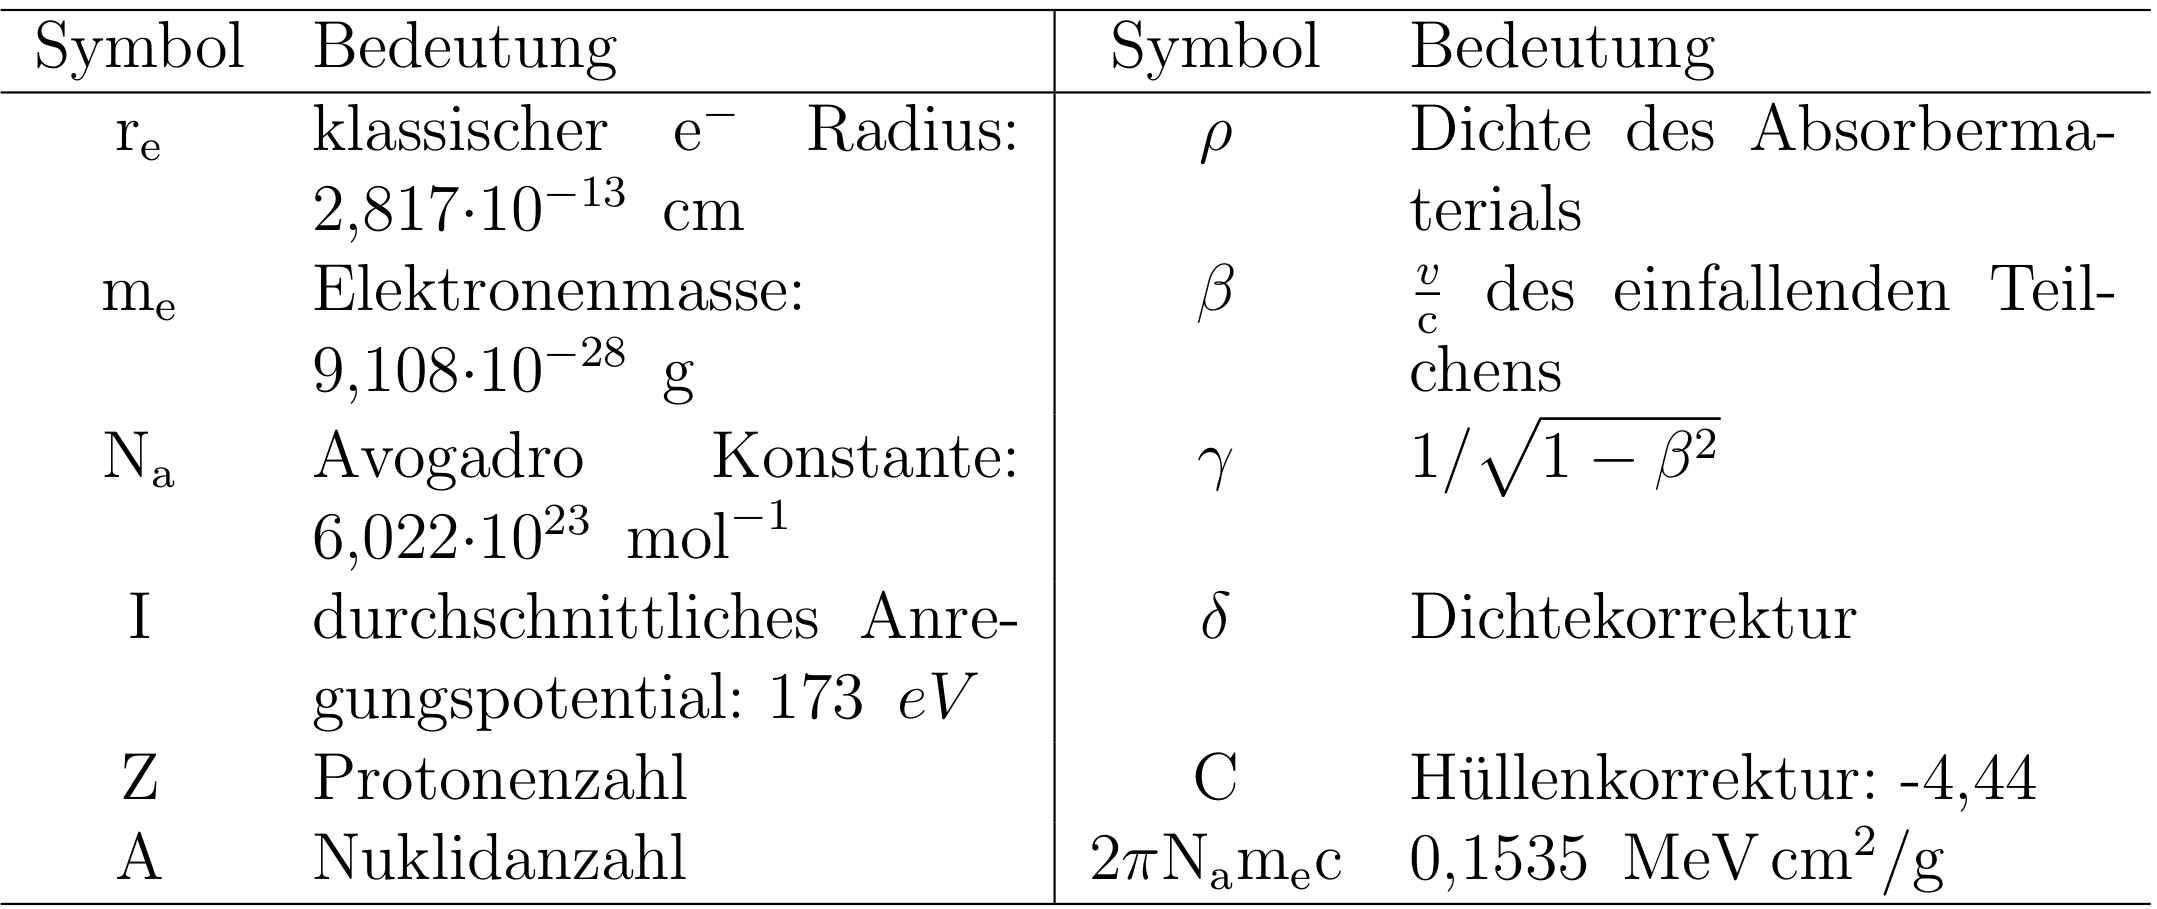
\includegraphics[width=0.8\textwidth]{images/Tabelle.png}
  \caption{Bestandteile der modifizierten Bethe-Bloch-Gleichung \cite{anleitung}.}
  \label{fig:tab}
\end{figure}
Typischerweise liegt die Energiedeposition von Elektronen in reinem Silizium bei
\SI{3.88}{\mega\electronvolt\per\centi\meter}.

\FloatBarrier
\subsubsection{Energiespektrum im Silizium-Detektor}
Bei hinreichender Dicke des Detektors ist das Spektrum der deponierten Energie eines
Elektrons aufgrund des zentralen Grenzwertsatzes durch eine Gaußverteilung gegeben.
Der hier verwendete Detektor erfüllt diese Bedingung bei einer Dicke von
\SI{300}{\micro\meter} jedoch nicht. Es gibt nicht genügend Wechselwirkungen
innerhalb des Detektors, um den zentralen Grenzwertsatz anwenden zu können.
Daher entspricht die Verteilung eher einer asymmetrischen Landau-Funktion.
Dies resultiert auch daraus, dass manche
Sekundärelektronen nicht innerhalb des Detektors gestoppt werden und daher
ein geringer Teil der deponierte Energie nicht korrekt bestimmt werden kann. Zudem
wird entlang der Fläche gestreut, was für einen langen Laufweg durch den Detektor
sorgt und sich daher ein langer Schwanz der Vertilung bilet.
Da die Energie der Elektronen des $\beta$-Zerfalls durch eine Verteilung beschrieben
werden können, beschreibt das Spektrum der deponierten Energie am besten eine Faltung zwischen
einer Gauß- und einer Landau-Funktion. Diese Verteilung ist in Abbildung \ref{fig:faltung}
dargestellt.
\begin{figure}[htb]
  \centering
  \includegraphics[width=0.5\textwidth]{images/Landau.png}
  \caption{Spektrum der Energiedisposition eines Elektron in einem dünnen Detektor. \cite{anleitung}}
  \label{fig:faltung}
\end{figure}
Dabei ist zwischen dem mittleren Energieverlust und dem wahrscheinlichsten Energieverlust
zu unterscheiden. Dies tritt durch die asymmetrische Landau-Funktion auf.


\FloatBarrier
\subsection{Pedestals und Noise}
\label{sec:Theorie_Noise}

Durch den Detektor und seine Ausleseelektronik enstehen Störsignale bzw. Rauschen,
sogennante Noise. Um dieses Rauschen zu Minimieren, wird die gemessene Anzahl von
Analog-Digital-Converter(ADC)-Counts für ein Signal $k$ und einen Streifen $i$
berechnet durch
\begin{equation*}
  \text{ADC}(i, k) = \text{P}(i) + \text{D}(k) + \text{Signal}(i, k).
\end{equation*}
Dabei beschreibt der Pedestal P($i$) den Mittelwert der ADC-Counts für einen
einzelnen Streifen ohne zu erwartendes Signal und der Common Mode Shift D($k$)
eine Störung für alle Streifen während eines Events. P($i$) und D($k$) berechnen
sich wie folgt:
\begin{align}
  \text{P}(i) &= \frac{1}{N} \sum_{k=1}^N \text{ADC}(i, k)
  \label{eqn:pedestal} \\
  \text{D}(k) &= \frac{1}{128} \sum_{i=1}^{128} \left(\text{ADC}(i, k) - \text{P}(i) \right)
  \label{eqn:common-mode}
\end{align}
Wird nun eine Nullhypothese für das Signal angesetzt (Messung ohne Quelle),
so lässt sich durch einen Root Mean Square die Noise der einzelnen Streifen berechnen:
\begin{equation}
  \text{Noise}(i) = \sqrt{ \frac{1}{N-1} \sum_{k=1}^N \left(\text{ADC}(i,k) - \text{P} (i) - \text{D}(k)\right)^2 }
  \label{eqn:noise}
\end{equation}
Bei einer Aufnahme von Daten wird ein \textit{Signal-to-Noise-Cut} durchgeführt,
um das Rauschen so gut wie möglich herausfiltern zu können. Dies geschieht
dadurch, dass ein Verhältnis zwischen den gemessenen Signalen des $\beta$-Strahlers
und dem Rauschen der Streifen gebildet wird. Ist dieses Verhältnis größer als 5,
so wird ein Trigger gesetzt und die Daten werden zur Messung herangezogen. Bleibt
das Verhältnis jedoch unter 5, so werden die Daten verworfen.

\subsection{Clustering}
\label{sec:Clustering}
Zuletzt muss noch auf die Bildung von Clustern eingegangen werden. Cluster
bezeichnen dabei das Messen eines Signals in mehreren Streifen. Grundlegend
gibt es drei Effekte, die auftreten können.
\begin{enumerate}
  \item \textit{Charge Sharing}: Hier trifft ein geladenes Teilchen genau
  zwischen zwei Streifen auf. Draufhin messen beide Streifen das Signal.
  \item \textit{Crosstalks}: Durch ein Signal in der Ausleseelektronik wird ein
  neues Signal an einem benachbarten Streifen gemessen.
  \item \textit{horizontale Events}: geht ein geladenes Teilchen schräg durch
  mehrere Streifen hindurch (mit einer Horizontalkomponente $\neq 0$), so gehen
  jegliche Ortsinformationen verloren. Für diese
  Ereignisse sind die Streifendetektoren nicht konstuiert worden.
\end{enumerate}
